\subsubsection{Xception}\label{xception}

To understand the Xception model, one must become familiar with depth-separable convolutions. This technique is a convolution operation that divides a standard convolution into two different stages to increase computational efficiency. Initially, a depth-wise convolution applies a single filter to each input channel. Subsequently, a point-wise convolution~-~characterized by a 1$\times$1 kernel~-~combines the outputs from the depth-wise step across the channels. This factorization significantly reduces the number of parameters and calculations and enables more efficient training. Batch normalization follows each convolution and promotes stable learning by normalizing the ReLU activations of the layer.

As seen in Figure~\ref{fig:xceptionArchitecture} the architecture of Xception, as detailed by \citep{chollet2017xception}, is structured into three primary flows. The entry flow prepares the network with initial convolutions and pooling to create condensed feature maps from the input images. It starts with two standard convolutions, followed by a series of separable convolutions that increase the depth while compressing spatial dimensions. This is achieved using a combination of 1$\times$1 convolutions for channel-wise feature processing and 3$\times$3 convolutions for capturing spatial information, each followed by max pooling to halve the feature map dimensions progressively. This step reduces the initial input image size from 299$\times$299$\times$3 to 19$\times$19$\times$728. Central to Xception's design is the middle flow, which repeatedly applies depthwise separable convolutions to process and refine the features. This part of the network is designed to be repeated eight times, allowing the model to learn increasingly complex patterns without a significant increase in computational cost. The dimensions do not get affected in this stage. The exit flow then expands the feature maps through additional separable convolutions, incorporating a mix of channel-wise and spatial feature extraction before concluding with global average pooling. This step reduces each map to a single vector, capturing the essence of the input data in a form suitable for classification. The network concludes with a logistic regression layer, such as softmax, to output the final class probabilities.

\begin{figure}[ht]
    \centering
    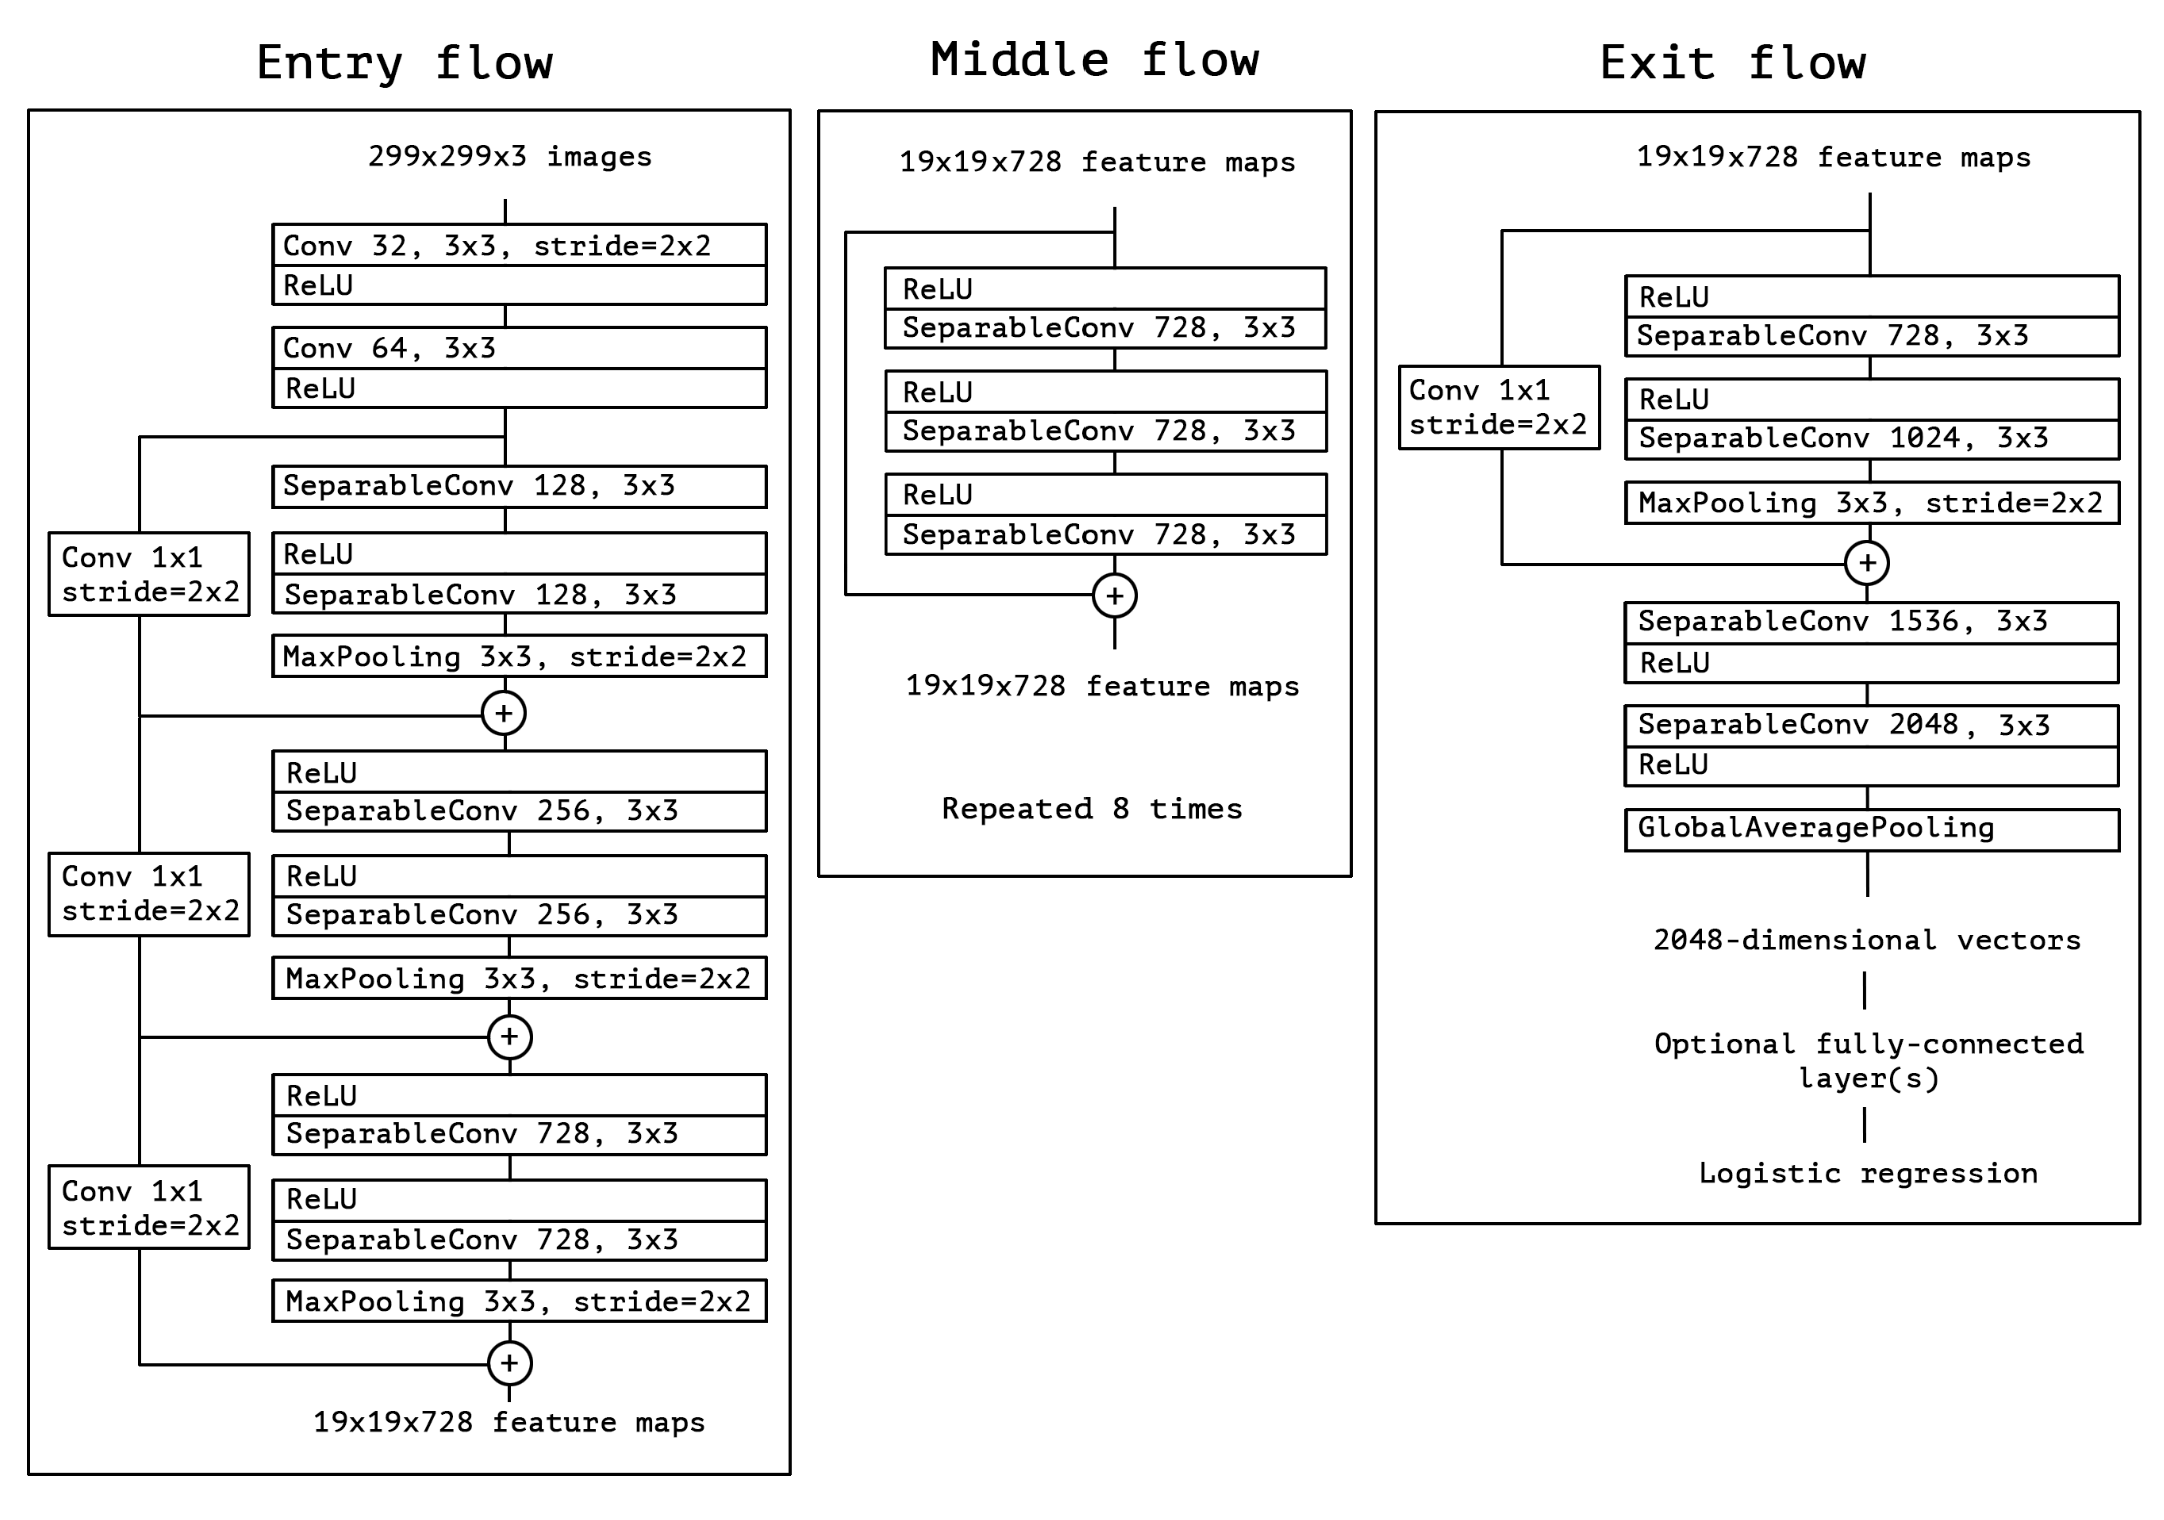
\includegraphics[width=0.9\textwidth]{figures/xception_architecture.png}
    \caption{Xceptions architecture as outlined by \citeauthor{chollet2017xception}.}\label{fig:xceptionArchitecture}
\end{figure}